\documentclass[border=0pt]{standalone}

% -----------------------------------------------------------------------------
% Springer-style modern package set
% -----------------------------------------------------------------------------
\usepackage{amsmath}
\usepackage{amssymb}
\usepackage{graphicx}
\usepackage{booktabs}
\usepackage{microtype}
\usepackage[style=numeric, backend=biber]{biblatex}
\usepackage{tikz}
\usetikzlibrary{calc, arrows.meta}
\usepackage{hyperref}
\usepackage{cleveref}

\begin{document}
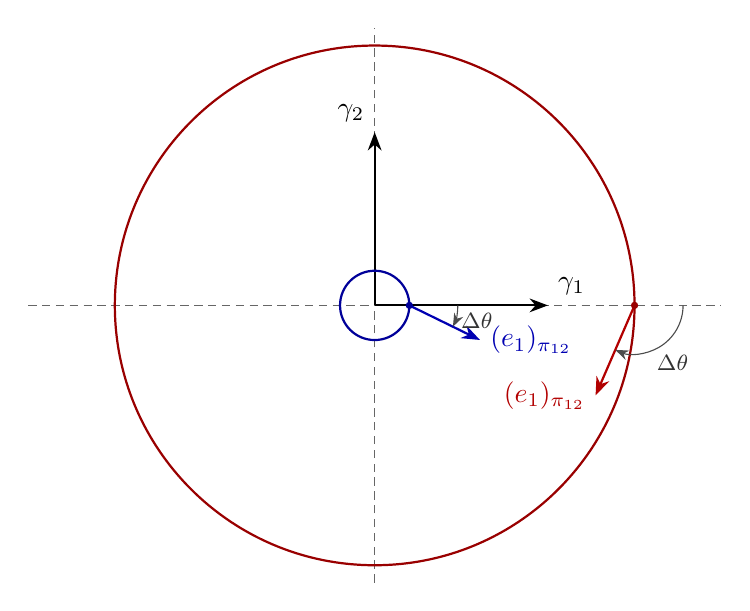
\begin{tikzpicture}[
  >=Stealth,
  scale=2.2,
  curveB/.style={thick, blue!60!black},
  curveR/.style={thick, red!60!black},
  vecB/.style={thick, ->, blue!70!black},
  vecR/.style={thick, ->, red!70!black},
  refVec/.style={thin, densely dashed, ->, black!50},
  axis/.style={thick, ->, black},
  axisExt/.style={thin, densely dashed, black!60}
  ]

  % ===========================================================================
  % KINEMATIC PARAMETERS
  % ===========================================================================

  % Low Velocity Regime (Blue)
  \def\aB{0.2}
  \def\gB{1.05}
  \def\dtB{25} % Scaled for visual clarity in the 2D projection

  % Relativistic Regime (Red)
  \def\aR{1.5}
  \def\gR{1.333}
  \def\dtR{120}

  % Uniform scaling factor for basis vectors
  \def\scl{0.45}

  % ===========================================================================
  % GEOMETRIC RENDERING
  % ===========================================================================

  % Origin and Spacetime Basis Axes
  \coordinate (O) at (0,0);

  % Extended coordinate axes
  \draw[axisExt] (-2.0, 0) -- (2.0, 0);
  \draw[axisExt] (0, -1.6) -- (0, 1.6);

  % Normalized unit basis vectors
  \draw[axis] (O) -- (1, 0) node[above right] {$\gamma_1$};
  \draw[axis] (O) -- (0, 1) node[above left] {$\gamma_2$};

  % Circular trajectories representing the projected invariant \gamma_{12} paths
  \draw[curveB] (O) circle (\aB);
  \draw[curveR] (O) circle (\aR);

  % Evaluation points at a full period (coinciding with the spatial axis)
  \coordinate (PB) at (\aB, 0);
  \coordinate (PR) at (\aR, 0);

  % ===========================================================================
  % VECTOR PROJECTIONS
  % ===========================================================================

  % Blue Precessed Frame Projections
  \coordinate (e1B) at ({\scl*cos(\dtB)}, {-\scl*sin(\dtB)*\gB});
  \coordinate (e2B) at ({\scl*sin(\dtB)}, {\scl*cos(\dtB)*\gB});

  \draw[vecB] (PB) -- ++(e1B) node[right] {$(e_1)_{\pi_{12}}$};
  \fill[blue!60!black] (PB) circle (0.6pt);

  % Red Precessed Frame Projections
  \coordinate (e1R) at ({\scl*cos(\dtR)}, {-\scl*sin(\dtR)*\gR});
  \coordinate (e2R) at ({\scl*sin(\dtR)}, {\scl*cos(\dtR)*\gR});

  \draw[vecR] (PR) -- ++(e1R) node[left] {$(e_1)_{\pi_{12}}$};
  \fill[red!60!black] (PR) circle (0.6pt);

  % ===========================================================================
  % HOLONOMY ANGLES
  % ===========================================================================

  % Calculate the exact visual angles encoding the gamma factor projection
  \pgfmathsetmacro{\visAngB}{atan2(-sin(\dtB)*\gB, cos(\dtB))}
  \pgfmathsetmacro{\visAngR}{atan2(-sin(\dtR)*\gR, cos(\dtR))}

  % Precession Angle Arc (Blue)
  \draw[thin, black!70, ->] ($(PB) + (0.28,0)$) arc (0:\visAngB:0.28);
  \node[font=\footnotesize, black!80] at ($(PB) + ({\visAngB/2}:0.40)$)
    {$\Delta\theta$};

  % Precession Angle Arc (Red)
  \draw[thin, black!70, ->] ($(PR) + (0.28,0)$) arc (0:\visAngR:0.28);
  \node[font=\footnotesize, black!80] at ($(PR) + ({\visAngR/2}:0.40)$)
    {$\Delta\theta$};

\end{tikzpicture}
\end{document}
